\section{Wavelet Transform Definitions}

As stated, the wavelet transform can be viewed from both a matrix
representation\cite{matrix01} and vector convolution. Both
representations provide means to use many linear algebra and abstract
algebra methods to prove theorems about wavelets.  Another form is a
convolution type of operation. Convolution wavelet transform methods
provide a simple computational method in general. Special case
convolution methods also exist, which allow even simpler algorithms to
perform wavelet transforms.

In the matrix form, a wavelet matrix is defined as a generalization of
a square orthogonal or unitary matrix which is a subset of a larger
class of rectangular matrices . This matrix harvests information for
defining a wavelet system.  Such matrices are defined in terms of
their rank and genus\cite{matrix01}.

It was Alfred Haar himself who defined an orthonormal wavelet matrix
in ``Zur Theorie der orthogonalen Funktionensystem Math Annual''
written in 1903. The said wavelet was named in honor of Alfred Haar,
the Haar Wavelet Matrix. A Haar Wavelet Matrix has a genus of
one. Such matrices have a one to one mapping to a general wavelet
matrix. Also, Haar Wavelet Matrices are equivalent to the
characteristic Haar Matrix. Lastly, a rank 2 Haar Matrix embodies all
geometric considerations\cite{matrix01}.

\section{Wavelets via Convolution}

Wavelets are defined in terms of average and difference components.
Each component can further be transformed to isolate properties of
each component.  Typically, each component has the form $S\rightarrow
(A|D)$ where $S$ is the original signal, $A$ is the average component, $D$
is the difference component and $(A|D)$ the signal $A$ concatenated with
$D$.  Each of these components are produced by an orthonormal basis.
Also, these components are produced such that the original can be
constructed easily from them.

Many mathematicians such as Walker\cite{walker}, use a form that
eliminates half of the values. Thus a form can be defined which has
the same number of elements as the original.  The rules for choosing
the member elements are dependent on the wavelet filter choice.


Another useful property of wavelets via convolution is the simplicity
of the operation. The general case works for all.  Such an algorithm
requires one nested loop as seen below:

\begin{tt}
\begin{tabbing}
$\forall i\in \lbrack 0,M)$ \\
\qquad $\forall j\in \lbrack 0,N)$ \\
\qquad \qquad n=i-j \\
\qquad \qquad if ($n\in \lbrack 0,M)$) \\
\qquad \qquad \qquad $y_{i\,}+=x_{n}\cdot h_{j\,}$
\end{tabbing}
\end{tt}

This filter simply equates to the mathematical function: $x\ast
h=\sum_{l}h(l)x(k-l)$, which is the convolution operation. As we can
see the operation is slightly less than $O(N^{2})$ . For practical
use, the filter is made smaller than the actual signal being
analyzed. In some cases, the filter may be much smalled than the
signal. Filter size matters in extracting features from the original
signal.

In the case of this convolution operator, the limit is actually $M$, not
$N$.  The value of $M$ is the size of the original signal. Since the
resulting vector is the same as the original, the vector is said to be
fully qualified. Only half of those values are necessary to
reconstruct the original (every other element).

To perform a wavelet transform via convolution, each signal is
convolved twice.
\[
A_{i}=A_{i-1}\ast V,
\qquad \qquad
D_{i\,}=A_{i-1}\ast W
\]
where 
\begin{itemize}
\item $V$ is the scaling wavelet vector,
\item $W$ is the differencing wavelet vector,
\item $A$ is the average vector (scaled vector),
\item $D$ is the difference component vector,
\item $\forall i\in \lbrack 1,L)$ and $A_{0}=f$ which is the
original signal, and
\item $L$ is the limit on the number resolutions that signal can have
based on the wavelet type.
\end{itemize}

\section{Class 2D Wavelet: Complete Form}

The convolution version can be used to derive a Wavelet Matrix.  For a
general case, it is simpler to use the convolution method.  The matrix
form becomes practical in repetitive special case applications.

The 2D transform has four components: the average, vertical,
horizontal, and diagonal. Two general computational means exist to
generate a one-resolution transform.  These can derive means for
performing many resolutions.

A complete transform method returns a result matrix which is the same
size as the source matrix. The result contains the four
components. Each component resides on 4 corners of the matrix. Given a
matrix $B$, the transform is to yield the following form:
\[ 
B \Rightarrow 
\left(
\begin{array}{cc}
H & D \\ 
A & V
\end{array}
\right)
\]
where $A$ is the average component, $H$ is the horizontal component,
$V$ is the vertical component, and $D$ is the difference
component. There is another form which is also used as an example:
\[
B \Rightarrow 
\left(
\begin{array}{cc}
A & V \\ 
H & D
\end{array}
\right)
\]
The first version is simple in concept, but provides a few more
possibilities for error and confusion.  Regardless of the case, the
four components have the following definitions:
\begin{enumerate}
\item Average component: produced by filtering the row vectors and the column vectors with the averaging filter.
\item Vertical Component:  produced by applying the average filter to the column vectors and the difference filter to the row vectors.
\item Horizontal component: produced by applying the average filter to the row vectors and the difference to the column vectors.
\item Diagonal component: produced by applying the difference filter to both the row and column vectors.  
\end{enumerate}

\subsection{Proof of Concept}
Two methods of convolving a matrix are easily conceived.  First is to
use 1D wavelet.  The other is to apply the convolution scheme
straight to the matrix. Included in the wavelet experiment are both.
Realistically, both can and do achieve the same result.  However, the
direct method achieves speed advantages by the lack of overhead.  The
direct method only stores a temporary vector resident in memory.  Also,
there are two fewer transfers per row and column.

\subsubsection{1D to 2D Method}

Both rows 1D and 2D and columns 1D and 2D transform are performed
similarly.  The obvious difference is the indexing of rows and
columns.

Given: 1D wavelet transform
source matrix

Algorithm: (Row Transform)

$\forall i \in rows$
\begin{itemize}
	\item $\forall j \in columns$
	
	\item $S[j] \leftarrow source[i][j] $
	
	\item $S \Rightarrow ^W  R$
\end{itemize}

This principle of this algorithm is simple.  Only three intuitive steps are necessary per row or column.  Two of these steps are array transfers (row/column transfer to an array).  These arrays are fed into the 1D transforms.  

However, the 1D wavelet transform itself includes a series of memory allocation and deallocation operations.  Each memory call is at the minimum a system call.  

\subsubsection {Vector - Matrix Method}
The principle of this algorithm is more complicated.  All functionality, such as convolution, is built into the method.  There are fewer calls and passing of structures to external functions to compute the transform.  

This method has a few givens.  The source matrix, the Haar average filter, and the Haar difference filter are given arguments.  The result argument is the return argument.    The transform signals sub-function row transforms and column transforms to perform the work.  

The algorithm is as follows for the row transform (and is similar for the column transform):  

$\forall i \in rows$
\begin{enumerate}
\item Initialize temporary array/vector to all zeros ($x$).
\item $\forall k \in columns $
\begin{enumerate}
\item $\forall l \in ha.Size$
%$
%x += 
%\begin{cases}
%S_{i,k-l} \ast hA_l, & \text{if $k-l \in columns$} \\ 
%0, & \text{otherwise}
%\end{cases}
%$

\end{enumerate}
\item $\forall k \in columns/2 $

$result_{i,k} = x_{2k+1} $  (In other words, odd split)

\item Initialize $x$ to all zeros.
\item $\forall k \in columns $
\begin{enumerate}
\item $\forall l \in hd.Size $

%$
%x +=$  
%\begin{cases}
%$S_{i,k-l} \ast hD_l$, & \text{if $k-l \in columns$} \\ 
%0, & \text{otherwise}
%\end{cases}


\end{enumerate}


\item $\forall k \in columns/2 $

$result_{i,k+columns/2} = x_{2k+1} $  (In other words, odd split)


\end{enumerate}

\subsection {Multiresolution}

The multiresolution wavelet transform and the inverse multiresolution transform resemble the vector-matrix version.  All functionality is built into this method.  However, there are structural changes.

The wavelet transform (multiresolution) uses private members of the class ($hA$, $hD$, $xD/yD$, $xA/yA$).  Both Haar filters are maintained this way.  Also both row and column transforms have average and difference myVector classes for temporary storage.   All of these members are allocated and destroyed by the wavelet transform method itself.   The simplified algorithm of the row transform is the following:
\begin{enumerate}
\item Initialize $xA$ and $xD$ to zero
\item $\forall k \in columns, \qquad \forall l \in filter$
\begin{itemize}
\item $n = k - l$
\item if ( $n \in columns $ )

	$xA_k = W_{i,n} * hA_l $
	
	$xD_k = W_{i,n} * hD_l $
	
	
\end{itemize}
\item Transfer back to W

	$W_i = xA|xD $
\end{enumerate}

And the column transform is represented by:
\begin{enumerate}
\item initialize $yA$ and $yD$ to zero
\item $\forall k \in rows, \qquad  \forall l \in filter$
\begin{itemize}
\item $n = k - l$
\item if ( $n \in columns $ )

	$yA_k = W_{i,n} * hA_l $
	
	$yD_k = W_{i,n} * hD_l $
	
	
\end{itemize}
\item Transfer back to $W$

	$W_j = yA|yD $
\end{enumerate}

Note: $W_i$ names the row vectors and $W_j$ names the column vectors, and $W_{i,j}$ is the element from the $i^{th}$ row and $j^{th}$ column.


%\subsection {Wavelet Transform: Quad Tree}
% The primary two addition to the wavelet transform in case of the Quad Tree variety is the tree and spare matrix.  The spare matrix is used to keep the transform operation separate during computation.  This may not be necessary in distributed versions.  

%The quad tree node has 9 elements side from links to 
%\begin {itemize}
%\item Energy (the section energy)
%\item coordinates for the upper left corner
%\item coordinates for the lower left corner
%\item coordinates for the upper right corner
%\item coordinates for the lower right corner 
%\end{itemize}

%The procedure for the quad tree wavelet transform involves loading the root node with its coordinates and the energy of the matrix.   This energy is used as an early stopping condition.  In the non-distributed form, it useful to load a temporary matrix global to the class/ object for the purpose of memory conservation, and system call conservation.  

%Given quad tree node, The steps are to compute the column wavelet transform followed by the row transform on matrix one and matrix two.  Following the computation of the wavelet transform, the energy for each segment must be computed.  If the energy limit (epsilon) or size limit has been reached, then stop procedure must be initiated.  Otherwise, the computation is continued for the 4 sub-components produced by the current wavelet transform.  

% The quad tree requires another feature in its structure, breadth first and depth first searching.  The purpose behind these searches is to extract the structure of the wavelet quad-tree transform and store it in an array.  This array can then be stored in a database, file, or passed to another procedure or returned to a calling procedure.  In the case of the leaves, this array can be made to store the actual matrix data, and its dimensions in another array.  

% The breadth first search requires a queue structure to hold pointers to the tree nodes.  First the root is put queue.  While the queue is not empty, the bread first search works on elements in the queue in a loop.  

% First step in the loop is to pop the element in the queue. Then stores that information.  Next the four children are inserted into the queue.  Then loop is repeated.  The only time that elements are not added to the queue is if they themselves are empty.  Eventually, the leaves are all reached, which have empty children.  This cause the queue to exhaust itself, and terminate the loop.  

% The depth first search essentially uses a stack, which implies that a recursive method can also be used.  The visit procedure is as follows:

% In particular there are two places where these traversal methods are necessary for the search, store, retrieval, transform, and inverse transform.  The first three are somewhat obvious.  The transform and inverse transform are not trivial.  

% In the depth first method, the transform is performed first for the average branches, starting at the root.  Once the average branch is transformed, the vertical branch is transformed by treating the first vertical child as its own root, and recursively repeating the transform.  This is again done for the horizontal and diagonal components.  

% The breadth first method first transforms the root, the same as the other methods.  Next, the branches formed by the transform are placed into a queue, and those elements are then transformed.  The step is repeated for subsequent transforms of each branch.  

% A hybrid approach takes the four branches after the transform uses size to evaluate whether to breadth first or depth first.  In the case of depth first, all four branches performed by separate threads of execution since the operations are independent of one another.  

% \subsubsection {Tree - Queue representation.  }
% For efficiency in speed, this implementation uses an array based tree and queue.  The reason is for ease of traversal, copying, storing, and retrieving.  The relation on the the array is as follows:
% \begin{itemize}
% \item $i_r = \frac{i_c -1}{4}$
% \item $ i_a = 4 i_r + 1$
% \item $ i_a = 4 i_r + 2$
% \item $ i_a = 4 i_r + 3$
% \item $ i_d = 4 i_r + 4$
% \end {itemize}

% Second is the construction of the tree data being stored.  For these experiments, wave-node keeps the energy of the matrix, the maximum value, the minimum value, the four corners, width, and width.

\subsection {Computational Cost}
The cost of this algorithm is computed first for each row and each column.  This value is used to compute the cost of the matrix. The cost of computing the matrix is used to compute the cost of the multiresolution steps.   Per row the cost is $3K$, where $K$ is the number of columns.  Per column the cost is $3L$, where $L$ is the number of rows.  For the whole matrix, one resolution costs $6KL$ operations to compute the wavelet transform.    Per resolution, the rows and columns shrink by $2^i $ for each resolution, i, performed.  The limit of this cost equals $12KL$ operations.  Thus, the cost is linear.  

%Stopped at this point April 10, 2003
\section{Results - 1D Wavelet Transform}
Testing of the 1D wavelet was performed on a sinusoidal wave form of 128 elements.  The given function has the equation shown in Figure \ref{sample}.

\[
y(n) = 10 \sin \left({n \over 128}\right) 
	- 5 \sin \left({n \over 64}\right) 
	+ 2 \sin \left({3 n \over 128}\right)
	- \sin \left({n \over 32}\right)
\]

\begin{figure}
\includegraphics [width=4in]{sample.jpg}
\caption{Sample function.  The $x$-axis is the array index (index $n$).  The $y$ value is simple -- the value $y(n)$. }
\label{sample}
\end{figure}


The first version of the 1D transform used the even elements of both convolutions to generate the wavelet transform.  These even elements came from the over-complete form and naturally allow the potential to have complete information.  However, in doing so, a fundamental flaw appears.

In order to evaluate the effectiveness of the wavelet transform three tests have been devised.  First,  energy equivalence is used to determine how much energy is retained in the transform from the original.    The general shape is used on a the first resolution to test if the average signal has the same general shape as the original.  Lastly, the inverse transform is used to recover the original signal.  A comparison is made between the original and the recovered signal.  

After one resolution, the transformed signal has the same energy as the original.  This is good since it allows the original to be recovered from the transform.  Also, the average component of the transform has the same shape as the original.  This is good.  However, the recovered signal is missing the last element.  Refer to Figure \ref{recoverEven}. The secret is in which elements are used from the over-complete to make the complete.  The over-complete in this project comes from the average component and difference which are simply the result of convolution.  

The convolution means is at the heart of the issue.  The convolution operator in this case starts with the first element of the filter against the first element of the signal.  In the simple Haar Wavelet case, there is a transformation pairing
\[
(S_i , S_{i-1}) \rightarrow A_i, \mbox{ and } (S_i , S_{i-1}) \rightarrow D_i .
\]
In this pairing with zero indexed signals, the odd indexed elements from the over-complete must be used to have all elements of the original accounted for.   

Also this produces a functional difference between wavelet inverse transform for odd and even versions.  The difference is slight; however, the last element is lost in the even indexed form.  

\begin{eqnarray*}
\mbox{Odd: } \qquad R_{2i} =(A_i - D_i ) \sqrt{1/2}, &\qquad& R_{2i+1}=(A_i + D_i ) \sqrt{1/2} \\
\mbox{Even: } \qquad R_{2i} =(A_i + D_i ) \sqrt{1/2}, &\qquad& R_{2i-1}=(A_i - D_i ) \sqrt{1/2} 
\end{eqnarray*}


%The even split  and analysis of this transform.  
\begin{figure}
\includegraphics [width=4in]{sample.jpg}
\caption{Recovered function.  The $x$-axis is the array index (index n).  The $y$ value is simply the value $y(n)$.  The function was recovered from an even indexed wavelet transform. }
\label{recoverEven}
\end{figure}

 
\begin{figure}
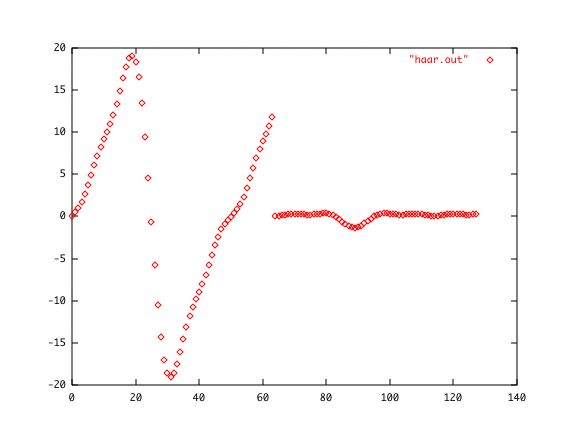
\includegraphics [width=4in]{recovered.jpg}
\caption{Recovered function.  The x-axis is the array index (index n).  The y value is simply the value y[n].  The function was recovered from an odd indexed wavelet transform. }
\label{recoverOdd}
\end{figure}

An odd indexed wavelet transform yields the same energy.  However, all of the values are accounted for.  Refer to Figure \ref{recoverOdd}.  

\section {Results: 2D Wavelet Transform }

A simple room picture shows the difference correct indexing produces in the wavelet transform and its inverse. The 1D to 2D method shows the incorrectly indexed case.  A correctly indexed version is shown in the vector-matrix method.  

The 1D to 2D method has a serious issue with memory leak errors (Macintosh OSX, using gcc 3.1).  Memory is allocated and deallocated quickly, and on some platforms shows up as an error.   On other platforms, the result is degraded performance (IRIX, SGI Octane2 using gcc 2.9).   An example image of 720 x 486 requires nearly 10 minutes to compute the wavelet transform by this method on an SGI Octane2.  However, this method does eventually return a correct result.  

The matrix-vector method also yields the correct result.  However, there is less memory overhead in this method as compared to the 1D to 2D method.  As a result, both the row wavelet transform and column wavelet transforms are performed more quickly, with fewer memory transfers and allocations.  Obviously, this also allows for the operation to be conducted almost entirely in cache memory on both the SGI Octane2 and Macintosh G4 based machines.  A Macintosh G3 based machine still requires main memory at a minimum to execute the same operation which yields a slower performance.  

A correct result must also be matched to a correct inverse method.  The indexing order matters.  The inverse transform method is a forward inverse transform method.  In the case of 1D to 2D transform, the ordering was reverse indexed (Figure \ref{rightWavepic}).  As a result of an error in indexing, ringing is seen on edges in this method(Figure \ref{rightDanRecovered}) for a case in point.  Caution is incredibly important when matching both forward and reverse indexing, since matching the mathematics to the actual ordering can be obscure and tricky.   

A correct result is shown in Figure \ref{selfRecover}.  In this case, the indexing was matched up and ringing is not present.  It is clear that the recovered image and the original (Figure \ref{rightDan}) are nearly indistinguishable.  

\begin{figure}[htb]
\begin{center}
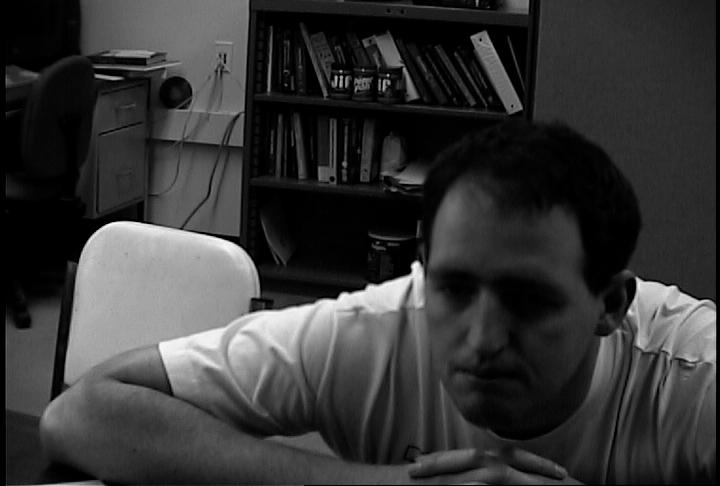
\includegraphics [width=4in]{rightDan.jpg}
\end{center}
\caption{Original Image.  This image is the original image. }
\label{rightDan}
\end{figure}

\begin{figure}[htb]
\begin{center}
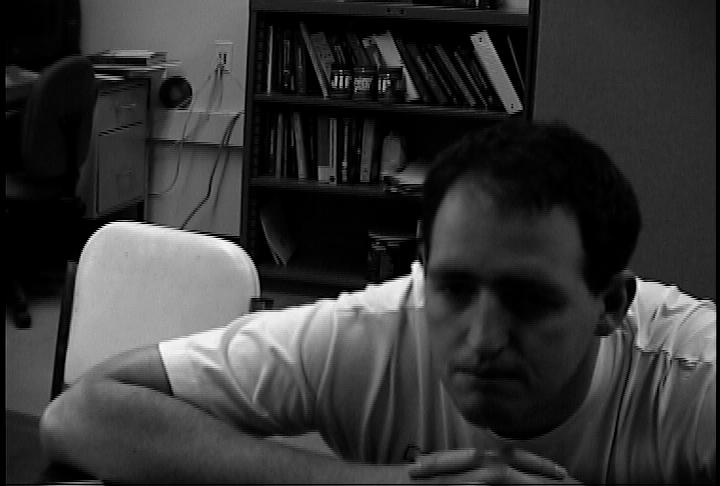
\includegraphics [width=4in]{revRecover.jpg}
\end{center}
\caption{Recovered Image.  This image is the recovered image.  Depending on whether the image was saved as a picture first can affect the white spots in the picture.  Ringing is also an issue.  }
\label{rightDanRecovered}
\end{figure}

\begin{figure}[htb]
\begin{center}
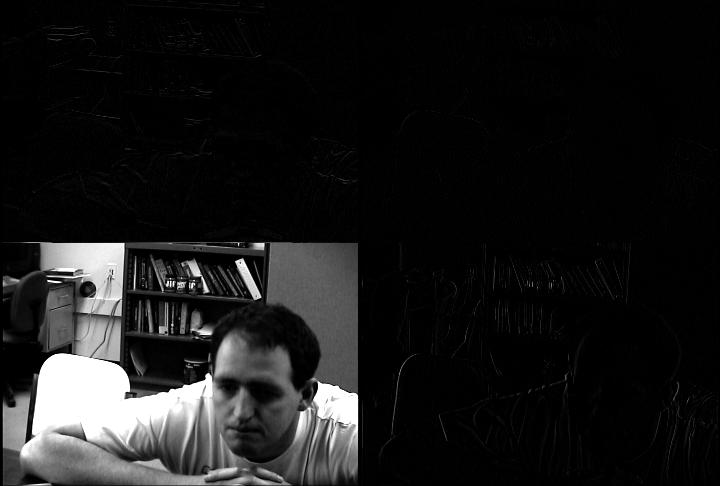
\includegraphics [width=4in]{revWavepic.jpg}
\end{center}
\caption{Wavelet Transform Image.  This image is divided in to average, horizontal, vertical and diagonal components. }
\label{rightWavepic}
\end{figure}

%Note: April 11, 2003:  Proofed up to this point

\begin{figure}[htb]
\begin{center}
\includegraphics [width=4in]{selfWavepic.jpg}
\end{center}
\caption{Wavelet Transform Image.  This image is divided in to average, horizontal, vertical and diagonal components, using the vector-matrix version. }
\label{wavepic}
\end{figure}

\begin{figure}[htb]
\begin{center}
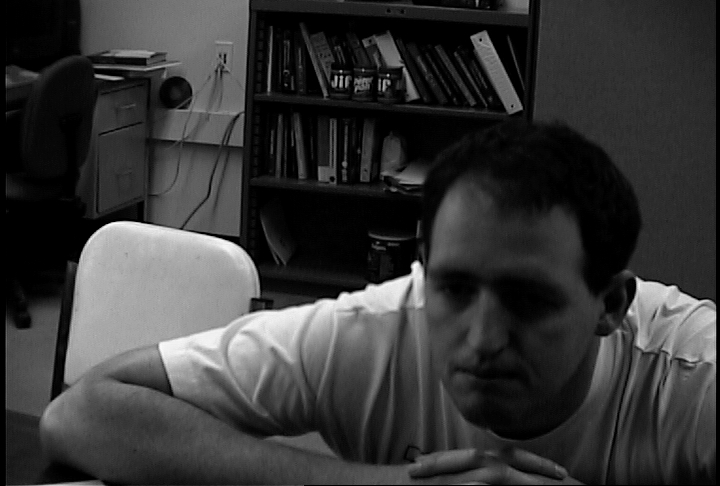
\includegraphics [width=4in]{selfRecover.jpg}
\end{center}
\caption{Recovered Image (Vector-Matrix Method).  This image is the recovered image.  This version avoids the ringing by using the vector-matrix version which is more aligned for the inverse wavelet transform.  }
\label{selfRecover}
\end{figure}

\subsection {Multiresolution}
The expected result is a picture within a picture.  Each average component has a further transform on it.  The three resolution transform has the form:
\[
W_3 = 
\left(
\begin{array}{cc}
\left(
\begin{array}{cc}
\left(
\begin{array}{cc}
A_3& V_3 \\ 
H_3 & D_3
\end{array} 
\right)
V_2 \\ 
H_2 & D_2
\end{array}
\right)
 & V_1 \\ 
H_1 & D_1
\end{array}
\right)
\]
Refer to Figure \ref{wavepicR3} for the image transform results.  

\begin{figure}[htb]
\begin{center}
\includegraphics [width=4in]{wavepic3R.jpg}
\end{center}
\caption{Wavelet Transform Image.  This image is divided in to average, horizontal, vertical and diagonal components using multiresolution wavelet transform.  Note the the average component was transformed one step further. }
\label{wavepicR3}
\end{figure}

\begin{figure}[htb]
\begin{center}
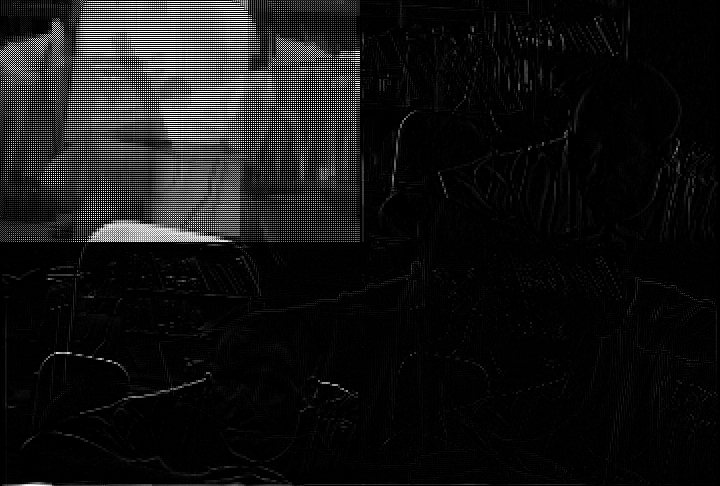
\includegraphics [width=4in]{recoverHid.jpg}
\end{center}
\caption{Recovered Image - Wrong Order (Multiresolution). This image shows a 2D wavelet transform after it was recovered out of order.  Obviously, the distortion is hideous.  }
\label{recoverHid}
\end{figure}

To obtain the inverse, an exact reverse procedure is necessary, otherwise the distortion is hideous.   The first attempt of the wavelet inverse transform was out of order, refer to Figure \ref{recoverHid} .  A correct picture was obtained during the second attempt.  Correct order yielded correct results, refer to Figure \ref{rightDanRecovered}.

\subsection {Threshold Filtering}
After a triple resolution, a 0.02 threshold will eliminate 81.1706 percent of elements in the original sample picture.  Also at this point, the effects of removing these elements becomes visually evident (Figure \ref{recover3R002}).  At a 0.01 threshold,  66.0205 percent of the elements are removed.  Visually, the recovered sample and the original appear to be the same (Figure \ref{recover3R001}).  At a threshold of 0.1, 92.9987 percent of the elements are reduced to zero.  However, the distortions are clearly visible at this level of thresholding (Figure \ref{recover3R010}).  Even at a threshold of 0.001 which is below the numerical precision of the original, 16.0814 elements are reduced to zero.  At a threshold of 0.002, 28.9683 percent is removed.  

Consequently after a triple resolution, nearly 29\% of the data was irrelevant for the image's brightness resolution (which also applies to color).  Subjective examination reveals that removing 60\% to 85\% of the data was not noticeable to human perception.  Which leaves only 15\% to 40\% of the data actually contributing or being necessary to reconstruct the image.   

\begin{figure}[htb]
\begin{center}
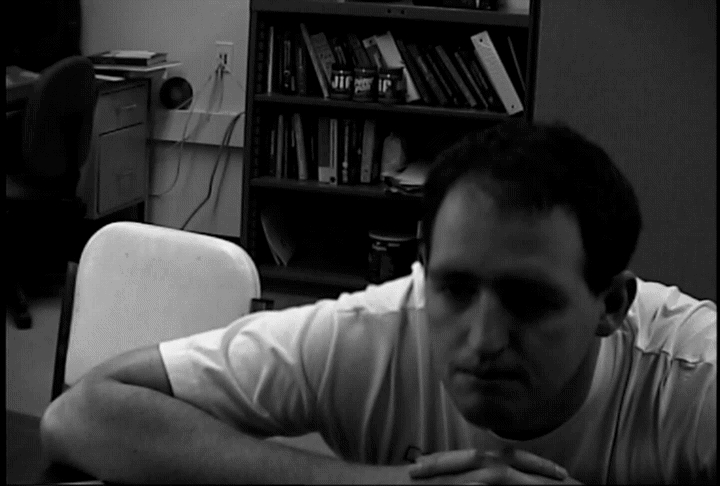
\includegraphics [width=4in]{recover3R002T.jpg}
\end{center}
\caption{Recovered Image - 2\% threshold (Multiresolution). This image had nearly 83\% of its elements removed in the triple resolution wavelet transform.  }
\label{recover3R002}
\end{figure}


\begin{figure}[htb]
\begin{center}
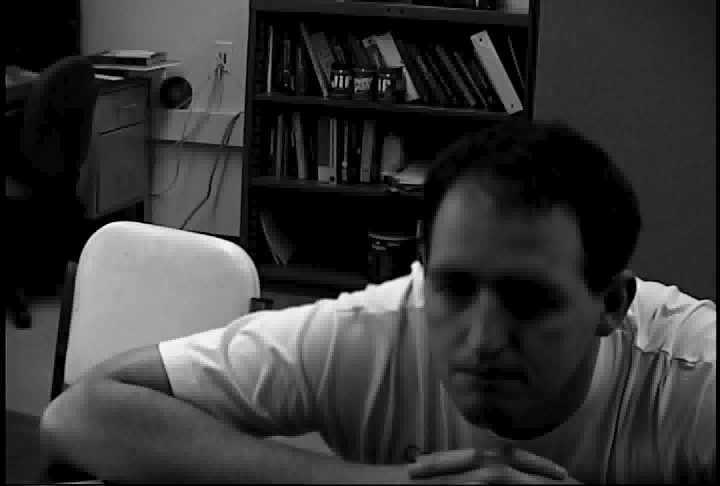
\includegraphics [width=4in]{recover3R010T.jpg}
\end{center}
\caption{Recovered Image - 10\% threshold (Multiresolution). This image had nearly 93\% of its elements removed in the triple resolution wavelet transform.  }
\label{recover3R010}
\end{figure}


\begin{figure}[htb]
\begin{center}
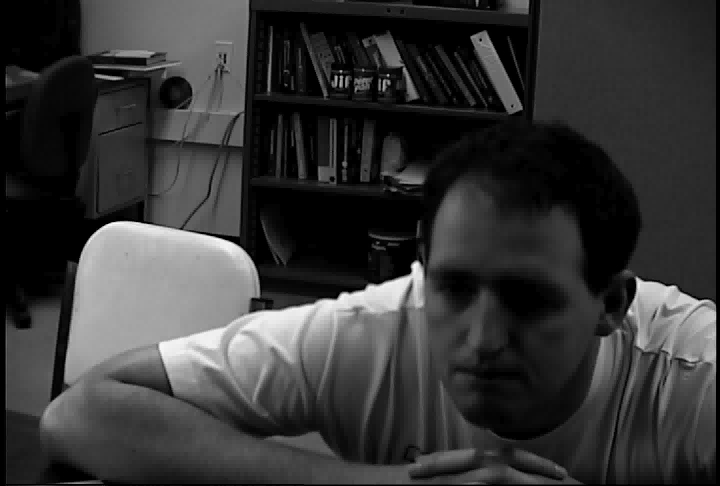
\includegraphics [width=4in]{recover3R005T.jpg}
\end{center}
\caption{Recovered Image - 5\% threshold (Multiresolution). This image had nearly 85\% of its elements removed in the triple resolution wavelet transform.    }
\label{recover3R005}
\end{figure}


\begin{figure}[htb]
\begin{center}
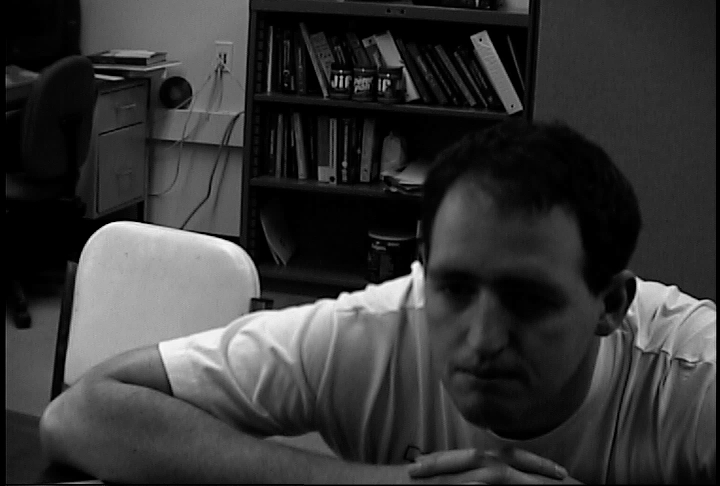
\includegraphics [width=4in]{recover3R001.jpg}
\end{center}
\caption{Recovered Image - 1\% threshold (Multiresolution).  This image had nearly 60\% of its elements removed in the triple resolution wavelet transform.   }
\label{recover3R001}
\end{figure}



%\begin{thebibliography}{99}
%\bibitem{matrix01}Howard L. Resnikoff. and Raymond O. Wells, Jr. \textsl {Wavelet Analysis: The Scalable Structure of Information}  copyright Springer-Verlag New York, Inc.  New York, NY 10010, USA, 1998
%\bibitem{walker}James Walker \textsl {A Primer on Wavelets and Their Scientific Applications}
%copyright Chapman \& Hall/CRC : Boca Raton, FL, USA, 1999
%\bibitem{tabor}Gavin Tabor \textsl {Wavelets - The Idiots Guide} http://monet.me.ic.ac.uk/people/gavin/java/waveletDemos.html
%\bibitem {graps} Amara Graps \textsl {Introduction to Wavelets} http://www.amara.com/current/wavelet.html 

%\end{thebibliography}
